\documentclass[tikz,border=3pt]{standalone}
\usepackage[utf8]{inputenc}
\usepackage[T1]{fontenc}
\usepackage{lmodern}
\renewcommand{\familydefault}{\sfdefault}
\usepackage{sansmath}\sansmath
\usepackage{chemfig}
\usepackage{pgfplots}\pgfplotsset{compat=1.18,/pgf/number format/use comma,/pgf/number format/1000 sep={.}}
\usetikzlibrary{arrows.meta,calc,positioning,decorations.pathmorphing,patterns}
% paleta del sitio
\definecolor{nar}{HTML}{E8680C}\definecolor{narc}{HTML}{FFB35C}\definecolor{hielo}{HTML}{FFF3E8}
\definecolor{tinta}{HTML}{1D1D1F}\definecolor{gris}{HTML}{6E6E73}\definecolor{lila}{HTML}{7C5CF0}
\definecolor{azul}{HTML}{2F6FD6}\definecolor{menta}{HTML}{17A673}\definecolor{coral}{HTML}{E8342A}
\begin{document}
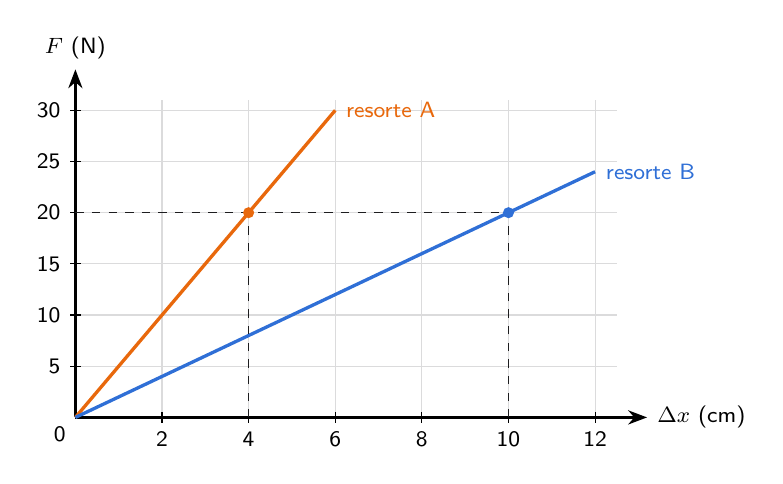
\begin{tikzpicture}[font=\footnotesize,>={Stealth[length=2.4mm]},x=0.55cm,y=0.13cm]
\foreach \y in {5,10,...,30} \draw[gris!25] (0,\y) -- (12.5,\y);
\foreach \x in {2,4,...,12} \draw[gris!25] (\x,0) -- (\x,31);
\draw[->,thick] (0,0) -- (13.2,0) node[right] {$\Delta x$ (cm)};
\draw[->,thick] (0,0) -- (0,34) node[above] {$F$ (N)};
\foreach \x in {2,4,...,12} \draw (\x,0.5) -- (\x,-0.5) node[below] {\x};
\foreach \y in {5,10,...,30} \draw (0.12,\y) -- (-0.12,\y) node[left] {\y};
\node[below left] at (0,0) {0};
\draw[very thick,nar] (0,0) -- (6,30) node[right] {resorte A};
\draw[very thick,azul] (0,0) -- (12,24) node[right] {resorte B};
\draw[dashed,tinta] (0,20) -- (10,20) (4,0) -- (4,20) (10,0) -- (10,20);
\fill[nar] (4,20) circle (2pt);
\fill[azul] (10,20) circle (2pt);
\end{tikzpicture}
\end{document}
